%=========================================================================
%=========================================================================
\chapter{DVD Contents}

Following files can be found on the attached DVD:

{\renewcommand{\arraystretch}{1.2}
\begin{table}[htbp]
	\centering
	\begin{tabularx}{1.0\textwidth}{lX}
		\textbf{/text} & Source files of this work (.tex), the figures and the final document (.pdf). \\
		\textbf{/poster} & The poster of this work presented at conference Excel@FIT 2016 (A1 format, .pdf). \\
		\textbf{/video} & The video  overviewing this work presented at conference Excel@FIT 2016 (.mp4, h264). \\
		\textbf{/paper} & The paper published at conference Excel@FIT 2016 (.pdf). \\
		\textbf{/ols/src} & Source code of the OLS divided into separate ROS packages (.cpp, .h, other auxiliary formats). \\
		\textbf{/ols/data} & Part of the meadow dataset (.bag). \\
		\textbf{/ols/doc} & The generated documentation of the source code (.html). \\
		\textbf{/misc/photos} & Various photographs of the OLS taken during development, rectification and testing (.jpg). \\
		\textbf{/misc/videos} & Various videos documenting the development and testing of the OLS (.mp4, h264). \\
		\textbf{/README.txt} & Text file including the description of the DVD contents, system requirements, building and running instructions and the usage manual. \\
	\end{tabularx}
	\label{tab:dvd_contents}
\end{table}%
}

%=========================================================================
%=========================================================================
\chapter{Usage of the OLS}

Table \ref{tab:ols_controls} summarizes the controls used to interact with the OLS. It is expected that the \textit{camera\_stream} window (see Section \ref{txt:user_interface}) is in focus.

% OLS controls.
\begin{table}[htbp]
	\centering
	\caption{OLS controls.}
	\begin{tabularx}{1.0\textwidth}{lX}
		\toprule
		\multicolumn{2}{c}{\textbf{KEYBOARD}} \\
		\midrule
		\multicolumn{1}{l}{\textbf{0-9 (alphanumeric)}} & \multicolumn{1}{l}{Switch among CUs.} \\
		\multicolumn{1}{l}{\textbf{left/right arrows}} & \multicolumn{1}{l}{Rotate the \gls{pt} unit around azimuthal axis.} \\
		\multicolumn{1}{l}{\textbf{down/up arrows}} & \multicolumn{1}{l}{Rotate the \gls{pt} unit around elevation axis.} \\
		\multicolumn{1}{l}{\textbf{4, 6 (numeric)}} & \multicolumn{1}{l}{Change the horizontal size of the bounding box.} \\
		\multicolumn{1}{l}{\textbf{2, 8 (numeric)}} & \multicolumn{1}{l}{Change the vertical size of the bounding box.} \\
		\multicolumn{1}{l}{\textbf{Y}} & \multicolumn{1}{l}{Select TLD tracker.} \\
		\multicolumn{1}{l}{\textbf{U}} & \multicolumn{1}{l}{Select BGFG tracker.} \\
		\multicolumn{1}{l}{\textbf{I}} & \multicolumn{1}{l}{select GT tracker.} \\
		\multicolumn{1}{l}{\textbf{Enter}} & \multicolumn{1}{l}{Start/stop tracking.} \\
		\multicolumn{1}{l}{\textbf{T}} & \multicolumn{1}{l}{Switch on/off regulation of the \gls{pt} motion.} \\
		\multicolumn{1}{l}{\textbf{S}} & \multicolumn{1}{l}{Switch stepper mode on (rotate \gls{pt} unit by steps).} \\
		\multicolumn{1}{l}{\textbf{C}} & \multicolumn{1}{l}{Switch continuous mode on (rotate \gls{pt} unit continusously).} \\
		\multicolumn{1}{l}{\textbf{Home}} & \multicolumn{1}{l}{Rotate the \gls{pt} unit so as to reach azimuth = 0 rad.} \\
		\multicolumn{1}{l}{\textbf{End}} & \multicolumn{1}{l}{Rotate the \gls{pt} unit so as to reach elevation = 0 rad.} \\
		\toprule
		\multicolumn{2}{c}{\textbf{MOUSE}} \\
		\midrule
		\multicolumn{1}{l}{\textbf{left button}} & \multicolumn{1}{l}{Start tracking the selected image region.} \\
		\toprule
		\multicolumn{2}{c}{\textbf{JOYSTICK/GAMEPAD}} \\
		\midrule
		\multicolumn{1}{l}{\textbf{axis-0}} & \multicolumn{1}{l}{Rotate the \gls{pt} unit around azimuthal axis.} \\
		\multicolumn{1}{l}{\textbf{axis-1}} & \multicolumn{1}{l}{Rotate the \gls{pt} unit around elevation axis.} \\
		\multicolumn{1}{l}{\textbf{axis-2}} & \multicolumn{1}{l}{Change the horizontal size of the bounding box.} \\
		\multicolumn{1}{l}{\textbf{axis-3}} & \multicolumn{1}{l}{Change the vertical size of the bounding box.} \\
		\multicolumn{1}{l}{\textbf{button-9 (start)}} & \multicolumn{1}{l}{Start/stop tracking.} \\
		\bottomrule
	\end{tabularx}
	\label{tab:ols_controls}
\end{table}

%=========================================================================
%=========================================================================
\chapter{Paper - Excel@FIT 2016}

\includepdf[pages={1,2,3,4,5,6,7,8}, offset=50 -45]{appendix/2016-ExcelFIT-paper.pdf}

%=========================================================================
%=========================================================================
\chapter{Poster - Excel@FIT 2016}

\begin{figure}[htp] 
	\centering {
		\vspace*{-1.5cm}
		\hspace*{-2.2cm}
		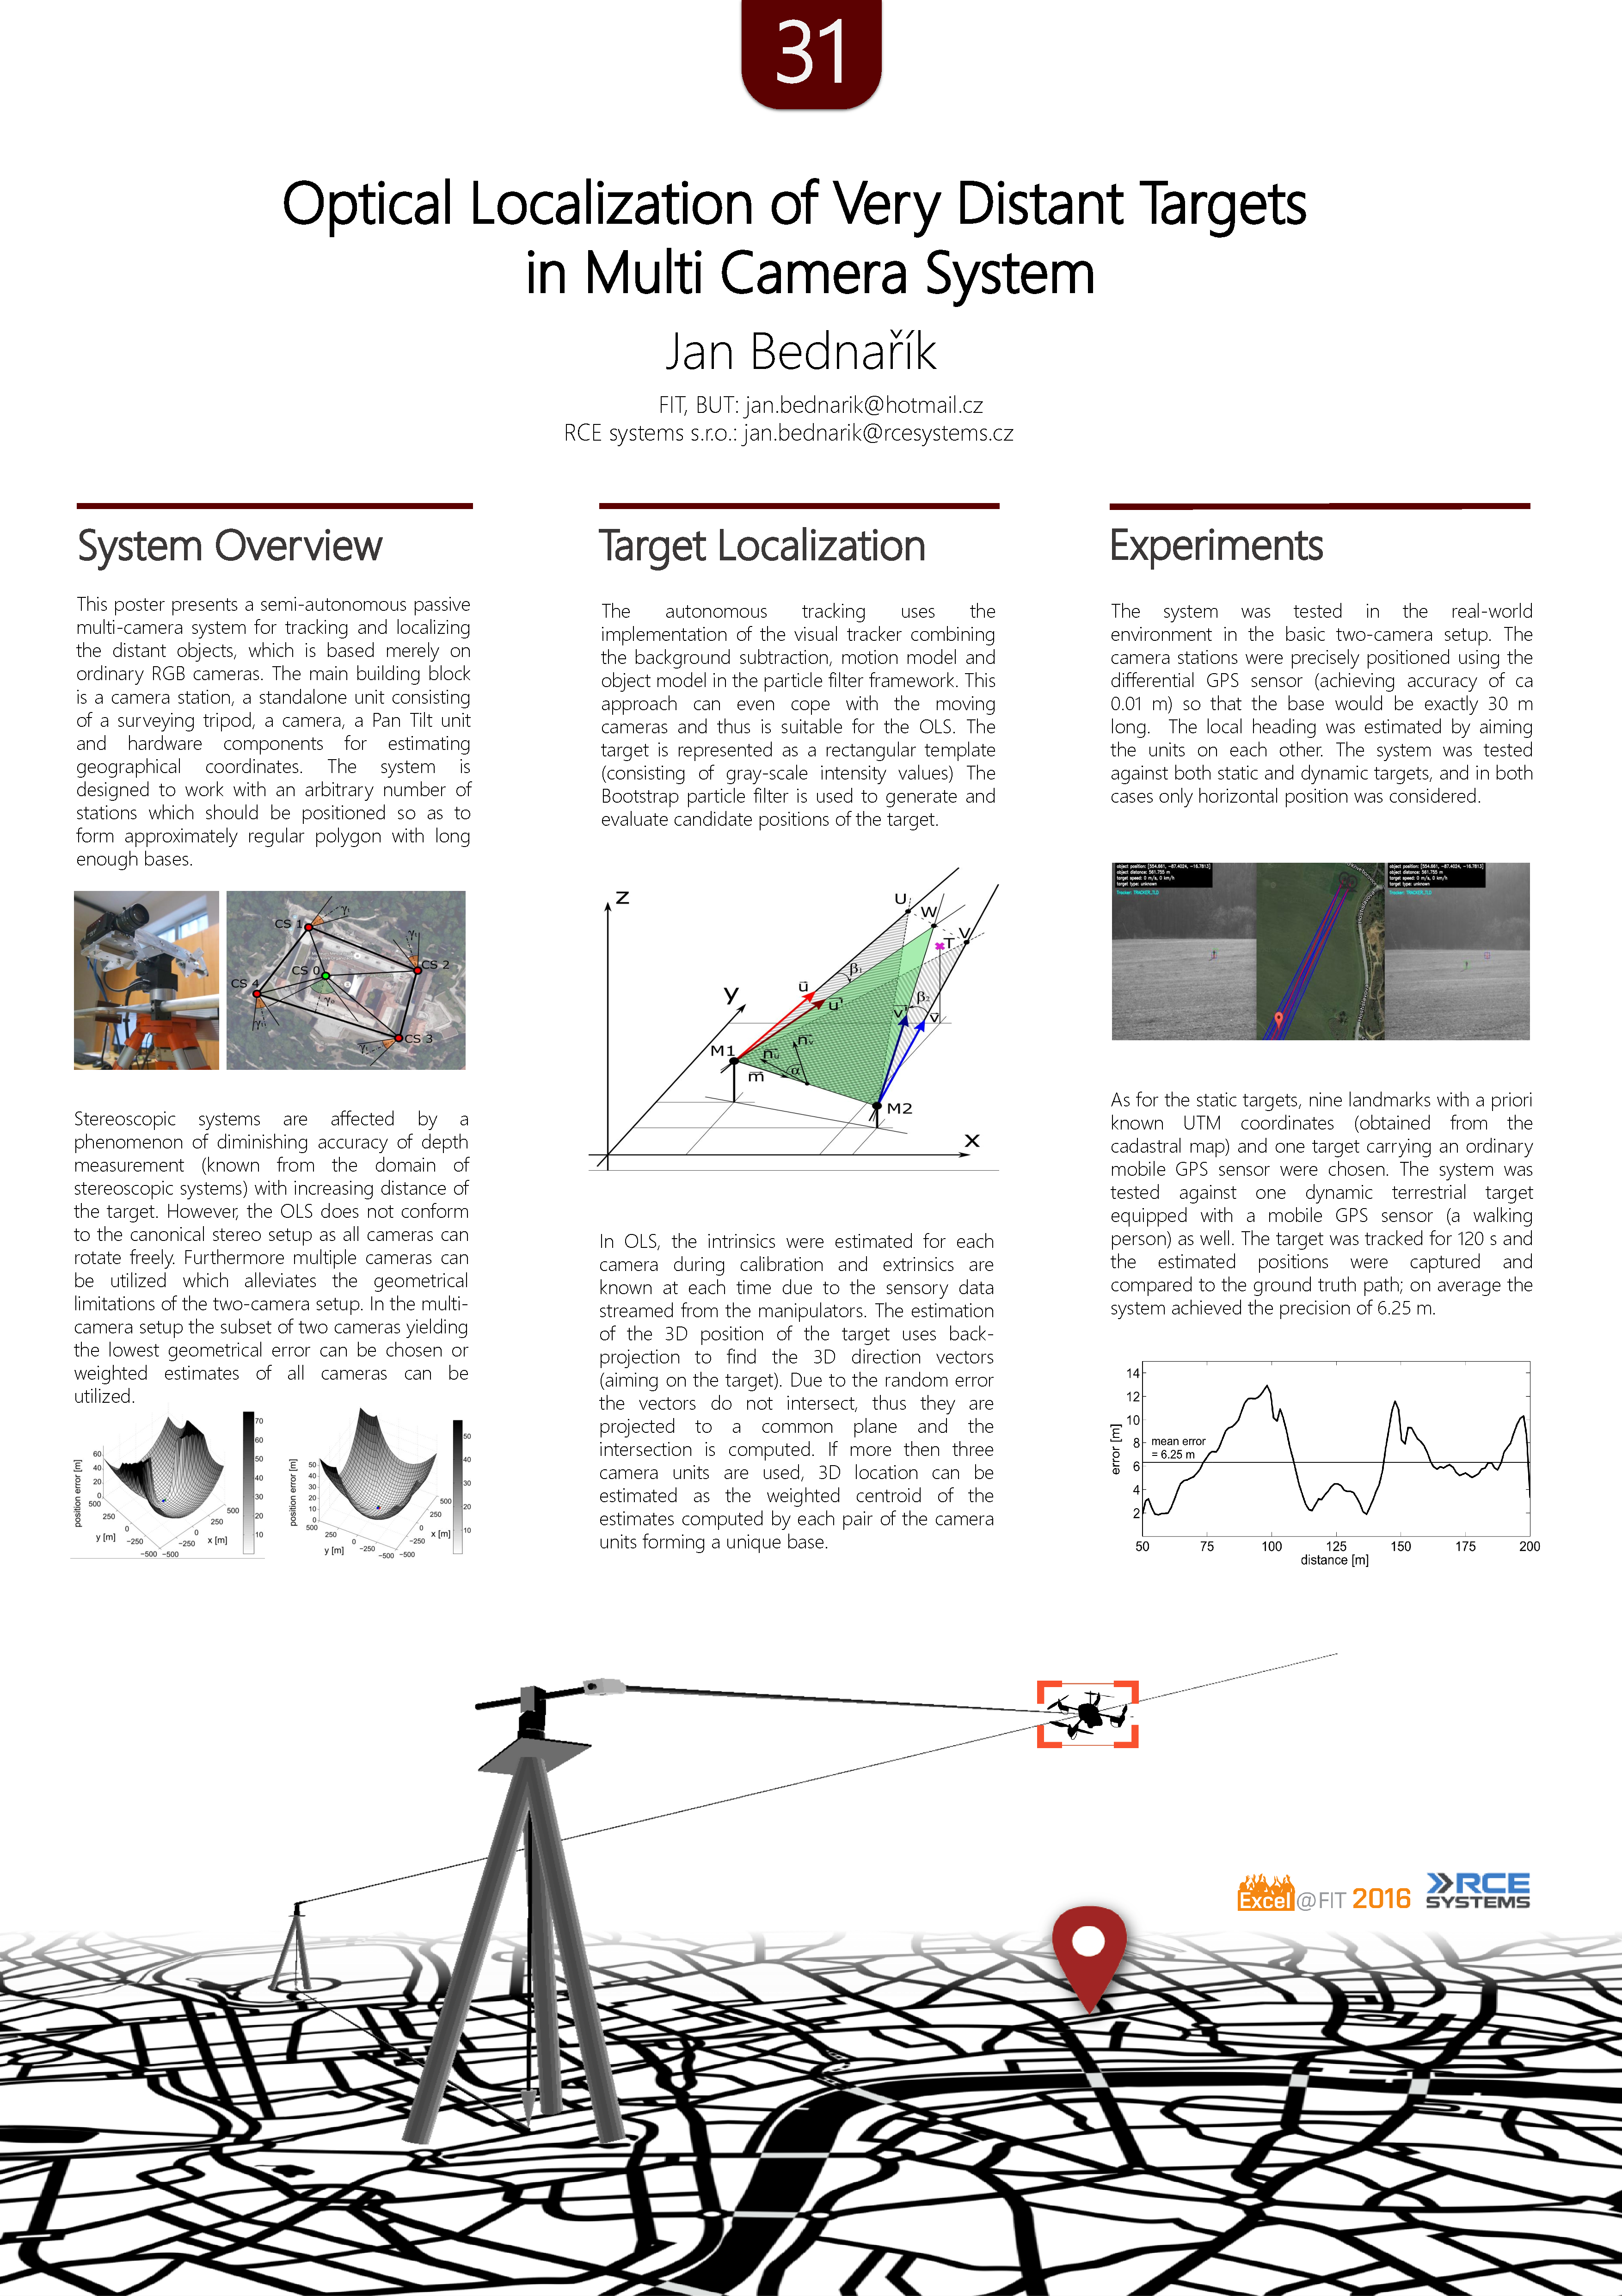
\includegraphics[scale=0.32]{appendix/2016-ExcelFIT-poster.pdf}
	}
\end{figure}